\documentclass[notes=hide,hyperref={dvipdfmx,pdfpagelabels=false}]{beamer}
\usepackage[xetex,dvipdfmx]{animate}
\title{Einführung in Sage - Einheit 7}
\subtitle{Funktionen, Grenzwerte, Funktionenfolgen, Grafiken}
\mode<article>
{
  \usepackage{fullpage}
  \usepackage{pgf}
  \usepackage[xetex]{hyperref}
  \setjobnamebeamerversion{beamer}
}

\mode<presentation>
{
  %\usetheme{Frankfurt}
 %\usetheme{My}
  \usetheme{Madrid}
  % or ...
%\usecolortheme{seagull}
  %\setbeamercovered{transparent}
  %\setbeamercovered{dynamic}
  % or whatever (possibly just delete it)
}
\usenavigationsymbolstemplate{}
\usefonttheme{structurebold}
\usepackage{multimedia}
%\usepackage{tikz}
\usepackage{fontspec,xunicode,xltxtra}

%\usepackage{polyglossia}
%\setdefaultlanguage[spelling=new, latesthyphen=true]{german}
%\setsansfont{DejaVu Sans}
%\setsansfont{Verdana}
%\setsansfont{Arial}
%\setromanfont{Linux Libertine O}
%\setsansfont{Linux Biolinum O}

\setbeamertemplate{footline}
{
\leavevmode
%\hbox{\begin{beamercolorbox}[wd=.5\paperwidth,ht=2.5ex,dp=1.125ex,
%leftskip=.3cm plus1fill,rightskip=.3cm]{author in head/foot}%
%    \usebeamerfont{author in head/foot}\insertshortauthor
%  \end{beamercolorbox}%
%  \begin{beamercolorbox}[wd=.5\paperwidth,ht=2.5ex,dp=1.125ex,leftskip=.3cm,
%rightskip=.3cm plus1fil]{title in head/foot}%
%    \usebeamerfont{title in head/foot}\insertshorttitle\hfill

\hfill\insertframenumber  \hspace{3pt}

%\inserttotalframenumber
%\hspace*{2ex}
%  \end{beamercolorbox}}%
  \vskip3pt%
}

\usepackage[ngerman]{babel}
\selectlanguage{ngerman}

%
% math/symbols
%
\usepackage{amssymb}
\usepackage{amsthm}
% \usepackage{latexsym}
\usepackage{amsmath}
%\usepackage{amsxtra} %Weitere Extrasymbole
%\usepackage{empheq} %Gleichungen hervorheben
%\usepackage{bm}
 %\bm{A} Boldface im Mathemodus

\usepackage{cellspace}
\setlength{\cellspacetoplimit}{2pt}
\setlength{\cellspacebottomlimit}{2pt}

%%%%%%%%%%%%%%%%%% Fuer Frames [fragile]-Option verwenden!
%Programm-Listing
%%%%%%%%%%%%%%%%%%
%Listingsumgebung fuer verbatim
%Grauhinterlegeter Text
%Automatischer Zeilenumbruch ist aktiviert
\usepackage{listings}
\definecolor{lgray}{gray}{0.80}
%\lstset{backgroundcolor=\color{lgray}, frame=single, basicstyle=\ttfamily, breaklines=true}
\lstnewenvironment{sage}{\lstset{backgroundcolor=\color{lgray},language=Python, emphstyle=\color{red}, frame=single, basicstyle=\ttfamily, breaklines=true,mathescape =true,escapechar=§}}{}


\usepackage{mydef}
%\usepackage{cmap} % you can search in the pdf for umlauts and ligatures
\usepackage{colonequals} %corrects the definition-symbols \colonequals (besides others)
\title{Einführung in Sage}
%
%\subtitle{Disputation} % (optional)

\author{Jochen Schulz}
% - Use the \inst{?} command only if the authors have different
%   affiliation.

\institute{Georg-August Universit\"at G\"ottingen \pgfimage[height=0.5cm]{../figures/unilogo3}}
% - Use the \inst command only if there are several affiliations.
% - Keep it simple, no one is interested in your street address.

\date{\today}

\subject{Sage}
% This is only inserted into the PDF information catalog. Can be left
% out. 

% If you have a file called "university-logo-filename.xxx", where xxx
% is a graphic format that can be processed by latex or pdflatex,
% resp., then you can add a logo as follows:

%\logo{\pgfimage[height=0.5cm]{figures/unilogo3}}


% Delete this, if you do not want the table of contents to pop up at
% the beginning of each subsection:

\AtBeginSection[]
{
  \begin{frame}<beamer>
    \frametitle{Aufbau}
    \tableofcontents[currentsection,currentsubsection]
  \end{frame}
}

\AtBeginSubsection[]
{
  \begin{frame}<beamer>
    \frametitle{Aufbau}
    \tableofcontents[currentsection,currentsubsection]
  \end{frame}
}



%%%%%%%%%%%%%%%%%%%
%Neue Definitionen
%%%%%%%%%%%%%%%%%%%

%Newcommands
\newcommand{\Fun}[1]{\mathcal{#1}}      %Mathcal fuer Funktoren
\newcommand{\field}[1]{\mathbb{#1}}     %Grundkoerper ?? in mathds

\newcommand{\A}{\field{A}}              %Affines A
\newcommand{\C}{\field{C}}              %Complexes C
\newcommand{\Fp}{\field{F}_{\!p}}       %Endlicher Koerper mit p Elementen
\newcommand{\Fq}{\field{F}_{\!q}}       %Endlicher Koerper mit q Elementen
\newcommand{\Ga}{\field{G}_{a}}         %Add Gruppenschema
\newcommand{\K}{\field{K}}              %Generischer Koerper 
\newcommand{\N}{\field{N}}              %Nat Zahlen
\newcommand{\Pj}{\field{P}}             %Projektives P
\newcommand{\R}{\field{R}} 		%Reelle Zahlen
\newcommand{\Q}{\field{Q}}              %Rationale Zahlen  
\newcommand{\Qt}{\field{H}}             %Quaternionen 
\newcommand{\V}{\field{V}}              %Vektorbuendel V
\newcommand{\Z}{\field{Z}}              %Ganze Zahlen

\newcommand{\fdg}{\;|\;}                 %fuer die gilt

%Operatoren
\DeclareMathOperator{\Abb}{Abb}
%\usepackage{sagetex}

\begin{document}
\lstset{basicstyle={\lstbasicfont\footnotesize}}


\maketitle

\begin{frame}{Aufbau}
\tableofcontents
\end{frame}

% \begin{frame}{Übersicht}
% \begin{itemize}
% \item Funktionen
% \item Funktionen in MuPAD
% \item Grenzwerte und Stetigkeit
% \item Funktionenfolgen
% \item Grafik
% \end{itemize}
% \end{frame}

%===================================================
\section{Funktionen}
%==================================================

\begin{frame}{Funktionen}
Man spricht von einer (reellen) {\color{red} Funktion}, wenn ein {\color{red}
  Definitionsbereich} $D \subset \mathbb{R}$, $D \neq \emptyset$
  gegeben ist und eine Vorschrift, die jedem $x \in D$ in eindeutiger
  Weise eine reelle Zahl $f(x)$ zuordnet. Man schreibt 
\[f: \ D \ \rightarrow \ \mathbb{R}.\]

Die Menge $f(D)$ ist die Menge aller rellen Zahlen, die als Werte der
Funktion vorkommen. Die Menge $f(D)$ wird als {\color{red} Wertebereich} bezeichnet. Der
{\color{red} Graph} einer Funktion ist die Menge aller Punkte 
\[ \{ (x,f(x)) \in \mathbb{R}^2 \;|\; x \in D\}. \]
\end{frame}

\begin{frame}[fragile]{Verknüpfungen}
Seien $f$ und $g$ Funktionen mit einem gemeinsamen Definitionsbereich. Dann
definiert man:
\begin{itemize}
\item Summe: $(f+g)(x):=f(x)+g(x)$
\item Differenz: $(f-g)(x):=f(x)-g(x)$
\item Produkt: $(f\cdot g)(x):=f(x) \cdot g(x)$
\item Quotient: $(\frac{f}{g})(x):=\frac{f(x)}{g(x)}$, falls $g(x) \neq
0$ für alle $x \in D$ 
\end{itemize}

Sind $f:D_f \rightarrow \mathbb{R}$ und $g:D_g \rightarrow \mathbb{R}$
mit $f(D_f) \subset D_g$ so ist die Komposition definiert durch:
\[(g \circ f) (x):=g(f(x)).\] 
\end{frame}

\begin{frame}{Mehrere Veränderliche}
Ist $D \subseteq \mathbb{R}^n$ und $f : D \Rightarrow \mathbb{R}$ dann spricht man von
einer reellen Funktion in \alert{mehreren Veränderlichen}. Das Studium dieser Funktionen ist einer der Hauptinhalte der Diff2-Vorlesung.

\bigskip

Weiterhin können Funktionen auch Wertebereiche außerhalb der reellen Zahlen haben.
Z.B. 
\[f : D \Rightarrow \mathbb{R}^m.\]
 Im physikalischen Umfeld spricht man für $m=1$ dann von \alert{skalarwertigen Funktionen} und für $m>1$ von \alert{vektorwertigen Funktionen} oder \alert{Vektorfeldern}.
 
\end{frame}


\begin{frame}[fragile]{Abbildungen in Sage I}
In Sage wird eine Abbildung $f$ durch einen Ausdruck der Form {\color{red}\isage{f(x,y,...)}} gebildet, wobei $x$,$y$ die sind.
\begin{sagein}
f(x,y) = x^2+y^2; f
\end{sagein}
\begin{sage}
(x, y) |--> x^2 + y^2
\end{sage}
Die so definierte Funktion $f$ kann wie jede beliebige andere Funktion
aufgerufen werden. Funktionen haben den Datentyp \isage{expression}.
\begin{sagein}
_=var('a,b');f(a,b+1)
\end{sagein}
\begin{sage}
(b + 1)^2 + a^2
\end{sage}
\begin{sagein}
type(f)
\end{sagein}
\begin{sage}
<type 'sage.symbolic.expression.Expression'>
\end{sage}
\end{frame}

\begin{frame}[fragile]{Abbildungen in Sage II}
Wie gewohnt können Abbildungen addiert, subtrahiert, multipliziert und
dividiert werden:
\begin{sagein}
f(x) = 1/(1+x); g(x) = sin(x^2)
h = f+g; k = f*g; l = f/g
h(a),k(a),l(a)
\end{sagein}
\begin{sage}
(1/(a + 1) + sin(a^2), sin(a^2)/(a + 1), 1/((a + 1)*sin(a^2)))
\end{sage}
\end{frame}


\begin{frame}[fragile]{Kompositionen in Sage I}
Eine Komposition $f\circ g$ wird in Sage durch Ineinanderschachteln gelöst.
\begin{sagein}
f_g(x) = f(g); g_f(x) = g(f)
f_g(x), g_f(x)
\end{sagein}
\begin{sage}
(1/(sin(x^2) + 1), sin((x + 1)^(-2)))
\end{sage}
Mehrfaches Hintereinanderschalten $f(f(\cdots f(\cdot)))=f \circ \dots
\circ f(\cdot)$ wird in Sage ebenso druchgeführt.
\begin{sagein}
g4(x) = g(g(g(g))); g4
\end{sagein}
\begin{sage}
x |--> sin(sin(sin(sin(x^2)^2)^2)^2)
\end{sage}
\end{frame}

\begin{frame}[fragile]{Kompositionen in Sage II}
Diese Konstruktionen funktionieren auch mit Systemfunktionen:
\begin{sagein}
abs(real(-2+3*I))
\end{sagein}
\begin{sage}
  2
\end{sage}
Kompliziertere Funktionen können besser durch selbst definierte Funktionen erklärt
werden. Dies sind im Wesentlichen kleine Programme, die mit
\isage{def <func>():} beginnen (vgl. letzte Vorlesung).
\end{frame}

\begin{frame}[fragile]{Ausdrücke und Funktionen I}
Man kann in Sage wählen, ob man eine Funktion $f$ als Funktion oder
als Ausdruck darstellt. Die Funktionsauswertung ist i.A. allerdings unterschiedlich:
\begin{sagein}
Funktion(x) = 2*x*cos(x); Funktion(1)
\end{sagein}
\begin{sage}
  2*cos(1)
\end{sage}
\begin{sagein}
Ausdruck = 2*x*cos(x); Ausdruck(x=1)
\end{sagein}
\begin{sage}
  2*cos(1)
\end{sage}

\end{frame}

% \begin{frame}[fragile]{Ausdrücke und Funktionen II}
% Man kann durch Einsetzen aus einer Funktion einen Ausdruck machen:
% \begin{sagein}
% bool(Funktion=Ausdruck), bool(Funktion(x)=Ausdruck)
% \end{sagein}
% \begin{sage}
%   FALSE, TRUE
% \end{sage}
% Umgekehrt kann man aber auch aus einem Ausdruck eine Funktion
% machen. Dazu gibt es in der Bibliothek \isage{fp} den Befehl
% \isage{unapply}. 
% \begin{sagein}
% Ausdruck:=2*x*cos(x):
% (h:=fp::unapply(Ausdruck)), h(2), Ausdruck(2)
% \end{sagein}
% \begin{sage}
%   x -> 2*x*cos(x), 4*cos(2), 2*x(2)*cos(x)(2)
% \end{sage}
% \end{frame}

\begin{frame}[fragile]{Ausdrücke und Funktionen II}
Auch mehrere Veränderliche  sind möglich:
\begin{sagein}
_=var('y');Funktion2(x) = x+sin(y); Funktion2
\end{sagein}
\begin{sage}
 x |--> x + sin(y)
\end{sage}
\begin{sagein}
Funktion3(x,y) = x+sin(y); Funktion3
\end{sagein}
\begin{sage}
  (x, y) |--> x + sin(y)
\end{sage}
\end{frame}

% \begin{frame}[fragile]{Warnung im Umgang mit Funktionen}
% 
% {\color{red} Funktionen werden bei der Zuweisung nicht vollständig ausgewertet.}
% \begin{sagein}
% n:=1: f.n := x -> x^2+n
% \end{sagein}
% \begin{sage}
%  x -> x^2 + n
% \end{sage}
% \begin{sagein}
% f1(4); n:=0: f1(4)
%    17  16
% \end{sagein}
% \begin{sagein}
% (f.n := x -> x^2+n) $\text{dollar}$ n=4..5
% \end{sagein}
% \begin{sage}
%   x -> x^2 + n, x -> x^2 + n
% \end{sage}
% Ausweg: Verwendung des Operators {\color{red}\isage{-->}}
% \begin{sagein}
% (f.n := x --> x^2+n) $\text{dollar}$ n=4..5 
% \end{sagein}
% \begin{sage}
%   x -> x^2 + 4, x -> x^2 + 5
% \end{sage} 
% \end{frame}

%----------------------------------------
\section{Grenzwerte und Stetigkeit}
%----------------------------------------

\begin{frame}{Grenzwerte von Funktionen}
Sei $f$ eine Funktion mit Definitionsbereich $D$ und $a\in D$.
$f$ strebt für $x \rightarrow a$ gegen den {\color{red} Grenzwert} $b \in
\mathbb{R}$, wenn es zu jedem $\varepsilon >0$ ein $\delta >0$ gibt, so
dass für alle $x \in D\smallsetminus\{a \}$ mit $|x-a|<\delta$ gilt 
\[ |f(x)-b| < \varepsilon .\]
Der Grenzwert $b$ ist eindeutig bestimmt und man schreibt
\[ \lim_{x \rightarrow a} f(x) =b \mbox{ oder } f(x) \rightarrow b
\mbox{ für } x \rightarrow a. \]
Die Aussage überträgt sich sinngemäß auf $a=\pm \infty$.
\end{frame}

\begin{frame}{Bemerkungen}
\begin{itemize}
\item Folgenkriterium: Es gilt $ \lim_{x \rightarrow a} f(x) =b$
genau dann, wenn für \alert{jede} Folge $a_n \in D$ mit $a_n \neq a$ und $a_n \rightarrow a$
gilt $\lim_{n \rightarrow \infty} f(a_n)=b$.
\item Es gelten die üblichen Rechenregeln:
\begin{eqnarray*}
\lim_{x \rightarrow a}(f(x)+g(x)) &=&\lim_{x \rightarrow a} f(x) +
\lim_{x \rightarrow a} g(x) \\
\lim_{x \rightarrow a}(f(x) \cdot g(x)) &=& \lim_{x \rightarrow a}
f(x) \cdot \lim_{x \rightarrow a} g(x)
\end{eqnarray*}
wenn $\lim_{x \rightarrow a} f(x)$ \alert{und} $\lim_{x \rightarrow a}g(x)$
\alert{existieren}. 
\item Gilt $\lim_{x \rightarrow a} f(x)=b$, $\lim_{x \rightarrow b}
g(x)=c$ bei entsprechenden Definitionsgebieten für $f$ und $g$, so
folgt $\lim_{x \rightarrow a} g(f(x)) =c$.
\end{itemize}
\end{frame}

\begin{frame}[fragile]{Sage}
Grenzwerte werden in Sage mit dem Befehl \isage{limit} gebildet. 
Die Syntax des Befehls lautet
\begin{sagein}
expr.limit(x = a, dir=None, taylor=False)
limit(expr, x = a, dir=None, taylor=False)
\end{sagein}
Hierdurch wird der Grenzwert eines Ausdrucks mit Unbekannten $x$ an
der Stelle $a$ bestimmt. $a$ kann auch $\pm \infty$ sein (in
Sage \isage{infinity} oder \isage{oo}).\\
\bigskip
Ruft man \isage{limit} ohne \isage{option} auf, so wird der beidseitige
Limes berechnet. Falls \isage{dir='minus'} ist, wird der linksseitige
Limes berechnet; für \isage{dir='plus'} der rechtsseitige.
\end{frame}

\begin{frame}[fragile]{Beispiele in Sage I}
\begin{itemize}
\item Bestimme den Grenzwert $\lim_{x \rightarrow 0}
\frac{\sin(x)}{x}$
\begin{sagein}
limit(sin(x)/x,x=0)
\end{sagein}
\begin{sage}
  1
\end{sage}
\item Bestimme den Grenzwert $\lim_{x \rightarrow \infty}
\frac{\log(x)}{x}$
\begin{sagein}
limit(log(x)/x,x=infinity)
\end{sagein}
\begin{sage}
  0
\end{sage}
\item Bestimme den Grenzwert $\lim_{x \rightarrow \infty} \sqrt[x]{x}$
\begin{sagein}
limit(x^(1/x),x=infinity)
\end{sagein}
\begin{sage}
  1
\end{sage}
\end{itemize}
\end{frame}

\begin{frame}[fragile]{Beispiele in Sage II}
\begin{itemize}
\item Bestimme den Grenzwert $\lim_{x \rightarrow 0}
\sin(1/x)$
\begin{sagein}
limit(sin(1/x),x=0)
\end{sagein}
\begin{sage}
  ind
\end{sage}
Der Grenzwert existiert nicht. Sage gibt in diesem Fall \isage{ind} (indefinite aber beschränkt) zurück. 
\item Bestimme den Grenzwert $\lim_{x \rightarrow 0} |x|' $
\begin{sagein}
limit(diff(abs(x),x),x=0),
limit(diff(abs(x),x),x=0,dir='minus'),
limit(diff(abs(x),x),x=0,dir='plus')
\end{sagein}
\begin{sage}
  (und, -1, 1)
\end{sage}
\end{itemize}
\end{frame}

\begin{frame}{Stetigkeit}
Eine Funktion $f:D \ \rightarrow  \ \mathbb{R}$ heißt {\color{red} stetig an
der Stelle $x_0 \in D$}, wenn es zu jedem $\varepsilon>0$ ein $\delta>0$
gibt, so dass für alle $x \in D$ mit $|x - x_0| < \delta$ gilt
\[ |f(x)-f(x_0) | < \varepsilon .\]
Man sagt, dass $f$ {\color{red} stetig} ist, wenn $f$ an jeder Stelle $x_0
\in D$ stetig ist. \\
Sind $f$ und $g$ an $x_0$ stetig, so auch $f+g$, $f-g$, $f \cdot g$
und $\frac{f}{g}$ (falls $g(x_0) \neq 0$). 
\end{frame}

\begin{frame}{Wichtige Sätze I}
\begin{itemize}
\item Sei $f$ auf einem offenen Intervall $I$ definiert. $f$ ist an
$x_0 \in I$ genau dann stetig, wenn gilt
\[ \lim_{x \rightarrow x_0} f(x) = f(x_0). \]
\item Für $f:I \rightarrow \mathbb{R}$ und $g:J \rightarrow
\mathbb{R}$ gelte $f(I) \subset J$ und es seien $f$ an $x_0 \in I$ und
$g$ an $y_0=f(x_0)$ stetig. Dann ist $g \circ f$ an $x_0$ stetig.
\item Eine Funktion $f: D \rightarrow \mathbb{R}$ ist {\color{red}
linksstetig} bzw. {\color{red} rechtsstetig}, wenn $f|_{D\cap (-\infty,x_0)}$
bzw  $f|_{D\cap (x_0,\infty)}$ an $x_0$ stetig ist. Eine Funktion $f$
ist dann an $x_0$ stetig, genau dann wenn $f$ links- und rechtsstetig
an $x_0$ ist.
\end{itemize}
\end{frame}

\begin{frame}{Wichtige Sätze II}
\begin{itemize}
\item Eine stetige Funktion auf einem abgeschlossenen Intervall $I=[a,b]$
besitzt ein Maximum und ein Minimum.
\item Eine stetige Funktion $f$ auf einem abgeschlossenen  Intervall
$[a,b]$ nimmt in $I$ jeden Wert zwischen $f(a)$ und $f(b)$ an.
\item Potenzreihen $f(x)=\sum_{n=0}^\infty a_n (x-x_0)^n$ sind stetig
innerhalb ihres Konvergenzintervalls.
\end{itemize}
\end{frame}


\begin{frame}{Gleichmäßige Stetigkeit}
$f: D \rightarrow \mathbb{R}$ heißt {\color{red} gleichmäßig stetig auf $D$},
wenn es zu jedem $\varepsilon >0$ ein $\delta>0$ gibt, so dass für alle
Paare $x,x_0 \in D$ mit $|x - x_0|< \delta$ gilt
\[ | f(x)-f(x_0)| < \varepsilon. \]
\begin{itemize}
\item Die Exponentialfunktion ist auf jedem kompakten Intervall
gleichmäßig stetig (aber nicht auf ganz $\mathbb{R}$). 
\item $\log:(0,1) \rightarrow \mathbb{R}$ ist stetig aber nicht
gleichmäßig stetig.
\end{itemize}
\end{frame}

\begin{frame}[fragile]{Stetigkeit in Sage}
Für die Diskussion der Stetigkeit einer Funktion $f$ an einer Stelle
$x_0$ sei auf den Abschnitt zu Grenzwerten verwiesen. \\
\begin{sage}
limit(1/x,x=0,dir='plus') 
\end{sage}
\begin{sage}
 +Infinity
\end{sage}
\begin{sage}
 limit(1/x,x=0,dir='minus')
\end{sage}
\begin{sage}
 -Infinity
\end{sage}

\end{frame}


% (Komplexe) Unstetigkeitsstellen oder Definitionslücken können mittels
% \isage{discont} aufgespürt werden:
% \begin{sagein}
% discont(sin(1/x)*x,x)
% \end{sagein}
% \begin{sage}
%   {0}
% \end{sage}
% \begin{sagein}
% discont(exp(x),x)
% \end{sagein}
% \begin{sage}
%   {}
% \end{sage}
% \begin{sagein}
% discont(tan(x),x)
% \end{sagein}
% \begin{sage}
%   { 1/2*PI + X1*PI |  X1 in Z_ }
% \end{sage}
% \end{frame}
% 
% \begin{frame}[fragile]{Stetigkeit in MuPAD}
% \begin{sagein}
% discont(1/sin(x),x=-1..10)
% \end{sagein}
% \begin{sage}
%   {PI, 0, 2 PI, 3 PI}
% \end{sage}
% Vorsicht! Es werden komplexe Unstetigkeitsstellen gesucht!
% \begin{sagein}
% discont(ln(x),x)
% \end{sagein}
% \begin{sage}
%   (-infinity, 0]
% \end{sage}
% \begin{sagein}
% discont(ln(x),x,Dom::Real)
% \end{sagein}
% \begin{sage}
%   {0}
% \end{sage}
% \begin{sagein}
% ln(-2)
% \end{sagein}
% \begin{sage}
%   I PI + ln(2)
% \end{sage}
% \end{frame}

%----------------------------------------
\section{Funktionenfolgen}
%----------------------------------------

\begin{frame}{Funktionenfolgen}
Seien $f_n: D \ \rightarrow \ \mathbb{R}$, $n \in
\mathbb{N}$  rellwertige Funktionen auf  $D \subset \mathbb{R}$.
\begin{itemize}
\item $(f_n)_n$ heißt {\color{red} Funktionenfolge.}
\item Ist für jedes $x\in D$ die Folge $(f_n(x))_n$ konvergent, so wird durch 
\[ f(x):= \lim_{n \rightarrow \infty} f_n(x), \quad x \in D \]
die {\color{red} Grenzfunktion} $f:D \ \rightarrow \ \mathbb{R}$ definiert.
\item Man sagt $f_n$ strebe {\color{red} punktweise} auf $D$ gegen $f$.  
\item Durch $\sum_{i=1}^\infty f_i$ definierte {\color{red} Funktionenreihen}
sind spezielle Funktionenfolgen.
\end{itemize}  
\end{frame}

\begin{frame}{Beispiele: Grenzübergänge}
\begin{itemize}
\item $x^n \rightarrow 0$ auf dem Intervall $(-1,1)$.
\item $\left( 1+ \frac{x}{n} \right)^n \rightarrow \exp(x)$ auf $\mathbb{R}$.
\item Potenzreihen konvergieren innerhalb ihres Konvergenzradius.
\item {\color{red} Warnung} zum Vertauschen der Grenzprozesse für $x \in (0,1)$:
\[ \lim_{x \rightarrow 1} \lim_{n \rightarrow \infty} x^n =0 \neq 1 = 
  \lim_{n \rightarrow \infty} \lim_{x \rightarrow 1} x^n.\]  
\end{itemize}
\end{frame}

\begin{frame}[fragile]{Gleichmäßige Konvergenz}
\begin{Definition}
$(f_n)_n$ konvergiert {\color{red} gleichmäßig} auf $D$ gegen $f$, wenn es zu
jedem $\varepsilon >0$ ein $n_0 \in \mathbb{N}$ gibt, so dass für alle
$x \in D$ und $n\geq n_0$ gilt:
\[ |f_n(x) -f(x)| < \varepsilon.\]
\end{Definition}

\begin{Satz}
 Konvergiert $(f_n)_n$ gleichmäßig auf $D$ und existiert $\lim_{x
\rightarrow a} f_n(x)$ für $a\in D$, so gilt:
\[ \lim_{x \rightarrow a} \lim_{n \rightarrow \infty} f_n(x) = \lim_{n
\rightarrow \infty} \lim_{x \rightarrow a} f_n(x). \]
\end{Satz}
\end{frame}

\begin{frame}{Bemerkungen}
\begin{itemize}
\item Die Grenzfunktion einer gleichmäßig konvergenten Folge stetiger
Funktionen ist stetig.
\item Alle Aussagen übertragen sich analog auf Funktionenreihen: Ist $f_1, f_2, \ldots$, eine Folge von Funktionen auf $D \subseteq \mathbb{R}$ dann definiert
\[
 s := \sum_{n=1}^\infty f_n
\]
eine Funktionenreihe. Aussagen über die Funktionenreihe sind, analog zum Fall der \glqq normalen\grqq\ Reihen, Aussagen über die Folge der Partialsummen
\[
 s_k := \sum_{n=1}^k f_n.
\]
 
 
\end{itemize}
\end{frame}

%------------- ---------------------------
\section{Grafiken}
%----------------------------------------

\begin{frame}[fragile]{Grafiken}
\begin{itemize}
\item Die Funktionen \isage{<parametric_>plot()} und \isage{<parametric_>plot3d()} dienen
             zur Darstellung von Graphen von Funktionen mit einem
             bzw. zwei Argumenten. 
\item Grafiken werden im Notebook integriert.
\item 3D-Grafiken können interaktiv bearbeitet werden.
\end{itemize}
Grafiken werden nicht direkt erzeugt, d.h. ausgegeben, sondern erst werden 
{\color{red} grafische Objekte} wie Geraden, Funktionsgraphen oder Kurven 
erzeugt. 

Erst beim \isage{show()} oder falls sie in der letzten Zeile ohne Zuweisung stehen, werden die Objekte zu einer gemeinsamen {\color{red} grafischen
Szene} zusammengefaßt.

\end{frame} 

\begin{frame}[fragile]{plot()}
Skalare Funktionen $f1,f2,\ldots$, können durch den Befehl
\begin{sagein}
plot(f1,(x,a,b),optionen)
\end{sagein}
auf dem Intervall $x \in [a,b]$. Dabei ist die Angabe  von
\isage{(x,a,b)} optional. Beispiele:
\begin{sagein}
plot(x^2-1)
plot(sin(1/x),(x,-1,1))
plot(sin(1/x),(x,-1,1),adaptive_recursion=0)
\end{sagein}

\begin{sagein}
p = plot(sin(x),color='red',xmin=-pi,xmax=pi)
p += plot(cos(x),xmin=-pi,xmax=pi); p.show()
\end{sagein}
\end{frame}

\begin{frame}[fragile]{plot3d()}
Es werden Funktionen
$f:\mathbb{R}^2 \ \rightarrow \mathbb{R}$
grafisch dargestellt. (Genauer gesagt wird auch hier der Funktionsgraph als Teilmenge des $\mathbb{R}^3$ gezeichnet). Der Funktionsaufruf ist
\begin{sagein}
plot3d(f,(x,a,b),(y,c,d), plot_points=[nx,ny])
\end{sagein}
Hierdurch werden  Ausdrücke $f1, f2,\ldots$, auf 
$[a,b]\times [c,d]$ mit Hilfe  von $nx$ Gitterpunkten in $x$-Richtung
und $ny$ Punkten in $y$-Richtung dargestellt. 
\end{frame}

\begin{frame}[fragile]{Beispiele}
Plot von $f(x,y)=\sin(y^2+x)-\cos(y-x^2)$ auf $[0,\pi]^2$:
\begin{sagein}
f(x,y) = sin(y^2+x)-cos(y-x^2)
plot3d(f,(x,0,pi),(y,0,pi))
plot3d(f,(x,0,pi),(y,0,pi),plot_points=[10,10])
\end{sagein}
\medskip
Plot von $f(x,y)=\cos (20 \exp(-x^2-y^2 ))$ auf $[-1,1] \times [-1,1]$:
\begin{sagein}
g(x,y) = cos(20*exp(-x^2-y^2))
plot3d(g,(x,-1,1),(y,-1,1))
plot3d(g,(x,-1,1),(y,-1,1),plot_points=[80,80])
\end{sagein}
\end{frame}

\begin{frame}[fragile]{Grafische Szene}

\begin{sagein}
W = plot3d(sin(pi*((x)^2+(y)^2))/2,(x,-1,1),(y,-1,1), frame=False, color='purple', opacity=0.8) 
S = sphere((0,0,0),size=0.3, color='red', aspect_ratio=[1,1,1])
show(W + S, figsize=8)
\end{sagein}
\begin{center}
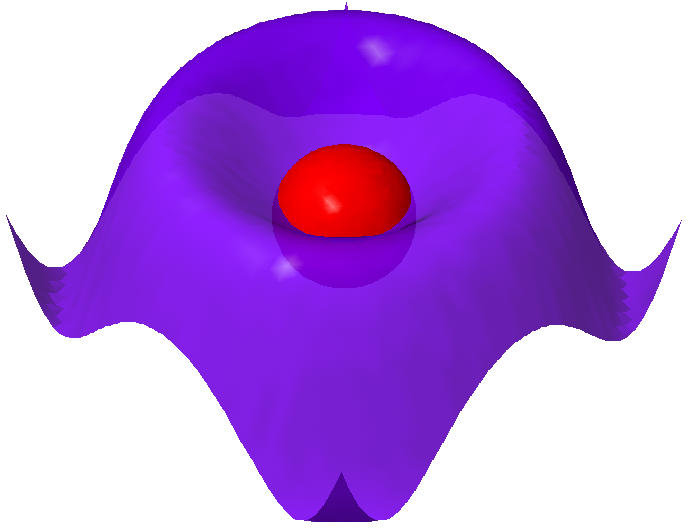
\includegraphics[width=7cm]{figures/ball.jpg} 
\end{center}
\end{frame}

\begin{frame}[fragile]{Ausgewählte Optionen für grafische Szenen}
\begin{tabular}{lp{8cm}}
\isage{aspect_ratio} & Verhältnis der Achsen (Breite/Höhe). $1$ für 1:1 Verhältnis. \newline
              {\color{blue} \isage{aspect_ratio = 2}}\\
\isage{figsize}    & Grösse des Bildes \newline
                  {\color{blue} \isage{figsize = [width, height]}}\\          
\isage{axes_labels} &  Tuple oder Liste der Achsenbeschriftungen \newline
{\color{blue} \isage{axes_labels = ('$x$','$y$')}}\\
\isage{gridlines} & Gitterlinien\newline
              {\color{blue} \isage{gridlines = True}}
\end{tabular}
\end{frame}

\begin{frame}[fragile]{Ausgewählte Optionen für grafische Objekte}
\begin{tabular}{lp{8cm}}
\isage{linestyle}  & Darstellung von Linien\newline
           (\isage{'-'} (solid), \isage{'-.'} (dashed), \isage{':'}) (dotted)\newline
                {\color{blue} \isage{linestyle = '.'}}\\
\isage{thickness}  & Linienstärke in mm\newline
              {\color{blue} \isage{thickness = 4}}\\
\isage{color}      & Zuweisung einer Farbe\newline
              {\color{blue} \isage{color='red'}}\\
\isage{plot_points}        & Anzahl Stützstellen\newline
              {\color{blue} \isage{plot_points  = [nx,ny]}} (2 Parameter)\\
\isage{alpha}  & Transparent\newline
     {\color{blue} \isage{alpha = 0.8}}\\
\end{tabular}
\end{frame}

\begin{frame}[fragile]{Zweidimensionale Kurven}
Eine Kurve des $\mathbb{R}^2$ in Parameterdarstellung sei gegeben durch Funktionen $x(t),y(t)$, also die Menge aller Punkte: 
\[
 \{(x(t),y(t)) \in \mathbb{R}^2 \;|\; t \in [a,b]\}.
\]
 Zum Beispiel ergibt sich der Graph einer Funktion $f(x)$, $x
\in [a,b]$ durch $t,f(t)$ mit  $t \in
[a,b]$. Der Befehl zum Erzeugen des Objekts ist 
\begin{sagein}
Objekt = parametric_plot([x,y],(t,a,b))
\end{sagein}
$x$ und $y$ sind Ausdrücke mit der Unbekannten $t$. Zusätzlich können
noch Optionen übergeben werden.
\end{frame}

\begin{frame}[fragile]{2D Kurven - Beispiele}
\begin{sagein}
_=var('t');f1 = parametric_plot([t,sin(t)],(t,0,2*pi),color='red')
f2 = parametric_plot([t,cos(t)],(t,0,2*pi),color='green')
f3 = parametric_plot([cos(t),sin(t)],(t,0,2*pi))
(f1+f2+f3).show(figsize=7)
\end{sagein}
\begin{center}
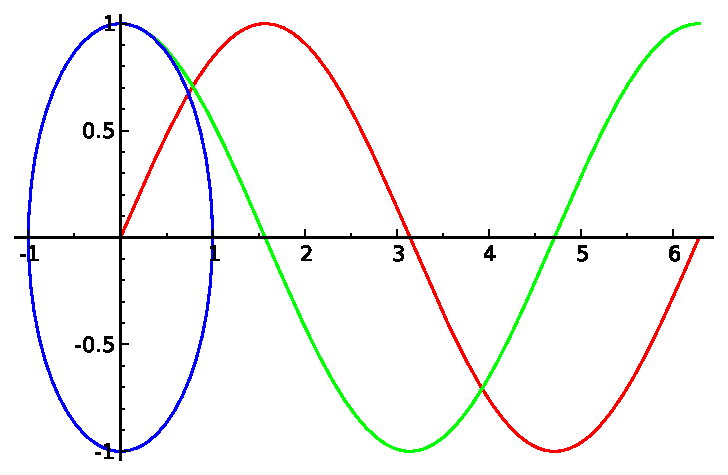
\includegraphics[width=7cm]{figures/parametric2d.pdf} 
\end{center}

\end{frame}

\begin{frame}[fragile]{2D Kurven - Beispiele}
\begin{sagein}
[parametric_plot([cos(t),sin(t)],(t,0,2*pi),plot_points=2*k+1,randomize=False,adaptive_recursion=0 ) for k in [2..10]]
\end{sagein}
\begin{center}
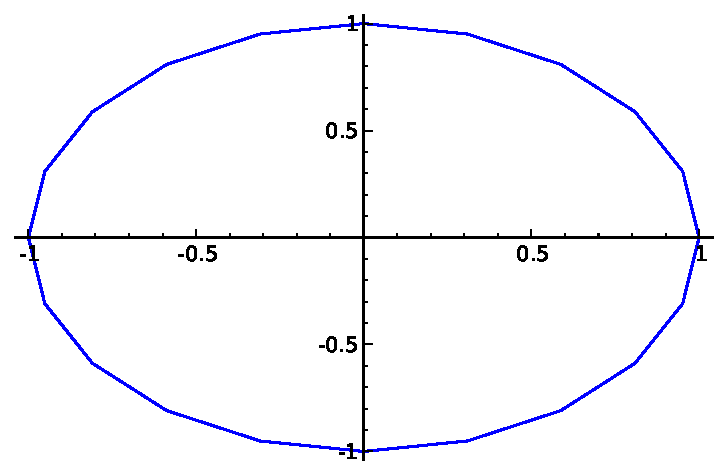
\includegraphics[width=7cm]{figures/parametric2d_2.pdf} 
\end{center}

\end{frame}

\begin{frame}[fragile]{Dreidimensionale Kurven}
Das Erzeugen einer dreidimensionaler Kurve, d.h. einer Kurve des $\mathbb{R}^3$ geschieht analog durch die Angabe von drei Funktionen $x(t),y(t),z(t)$:
\[
 \{(x(t),y(t),z(t)) \in \mathbb{R}^3 \;|\; t \in [a,b] \}.
\]
Der Befehl ist  
\begin{sagein}
Objekt = parametric_plot3d([x,y,z],(t,a,b))
\end{sagein}
$x$, $y$ und $z$ sind Ausdrücke mit der Unbekannten $t$. Zusätzlich können
noch Optionen übergeben werden. 
\end{frame}

\begin{frame}[fragile]{3D Kurven - Beispiel}
\begin{sagein}
parametric_plot3d([(1-t*t)*cos(99*t),(1-t*t)*sin(99*t),t], (t,0,1),plot_points=400)
\end{sagein}
\begin{center}
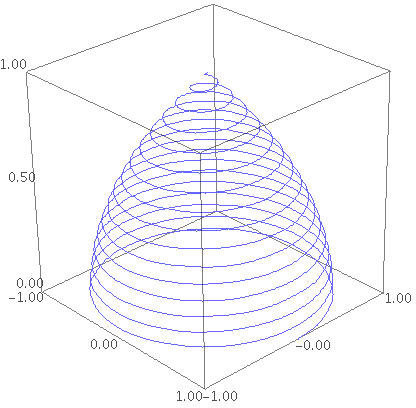
\includegraphics[width=7cm]{figures/parametric3d.jpg} 
\end{center}
\end{frame}

\begin{frame}[fragile]{Flächen}
\begin{itemize}
\item Typische dreidimensionale Grafikobjekte sind {\it parametrisierte Flächen}.
\item Die $x,y,z$ Koordinaten sind als Funktionen $x(t_1,t_2)$,
   $y(t_1,t_2)$, $z(t_1,t_2)$ zweier Parameter $t_1 \in [a,b]$ und $t_2 \in [c,d]$
   definiert. 
\item Beispielsweise lassen sich Graphen von Funktionen $f:[a
   ,b]\times [c,d]
   \ \rightarrow \ \mathbb{R}$ als Flächen
\[ x=t_1, \ y=t_2, \ z=f(t_1,t_2) \]
mit $a \leq t_1 \leq b, \ c \leq
   t_2 \leq d$ erklären.
\end{itemize}
\end{frame}

\begin{frame}[fragile]{Flächen}
\begin{itemize}
\item Die Oberfläche einer Kugel mit Radius $r$ ist gegeben durch:
\[ x=r \cos(t_1) \sin(t_2), \ y=r \sin (t_1) \sin (t_2), z =r
  \cos(t_2) \]
 mit $0 \leq t_1 \leq 2 \pi, 0 \leq t_2 \leq \pi.$ 
\item Flächen werden in Sage erzeugt durch
\begin{sage}
parametric_plot3d( [x(t1,t2), y(t1,t2), z(t1,t2)],(t1,a,b), (t2,c,d), Optionen):
\end{sage}
\end{itemize}
\end{frame}

\begin{frame}[fragile]{Flächen - Beispiel}
Ellipsoid-Oberfläche
\begin{sagein}
_=var('t1,t2');r=1
x=r*cos(t1)*sin(t2)
y=2*r*sin(t1)*sin(t2)
z=r*cos(t2)
parametric_plot3d([x,y,z],(t1,0,2*pi),(t2,0,pi),aspect_ratio=1)
\end{sagein}
\begin{center}
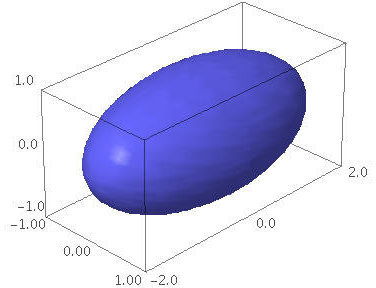
\includegraphics[width=5.5cm]{figures/surface.jpg} 
\end{center}

\end{frame}

\begin{frame}[fragile]{Konturen}
\begin{itemize}
\item Man kann für Funktionen $f:\mathbb{R}^2 \rightarrow \mathbb{R}$
auch zweidimensionale Grafiken erstellen.
\item Man zeichnet die Niveaulinien (wie die Höhenmeter auf einer
Landkarte), d.h. man sucht zu $c \in \mathbb{R}$ die Menge von Punkten
$(x,y)$ mit $f(x,y)=c$.
\item In Sage geschieht das mit dem Befehl
\begin{sagein}
contour_plot(f, (x,,), (y,,), contours=[c1,c2,...], options)
\end{sagein}
Dabei geben $c1,c2,\ldots$ die entsprechenden Niveaulinien an.
\end{itemize}
\end{frame}

\begin{frame}[fragile]{Konturen - Beispiel}
Wir betrachten die Funktion $\sin(4\pi x)y$ und zeichnen die Niveaulinien für $-0.5, 0, 0.5$. 
\begin{sagein}
contour_plot(sin(pi*4*x)*y,(x,-1,1),(y,-1,1),contours = [-0.5, 0, 0.5],fill=False,labels=True)
\end{sagein}
\isage{fill=True} würde die Flächen zwischen den Linien ausfüllen.
\begin{center}
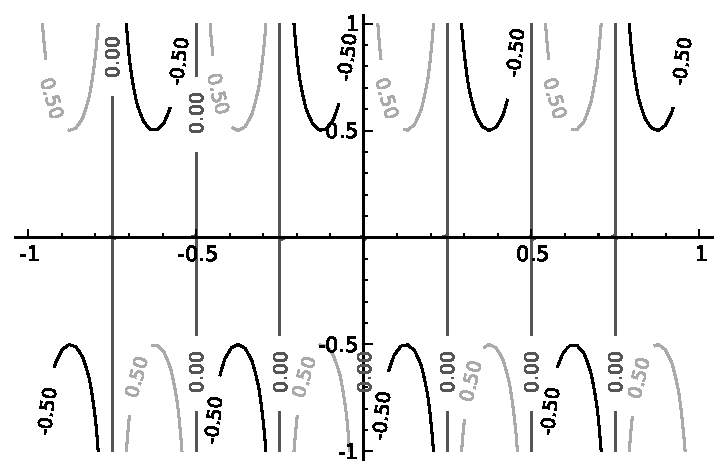
\includegraphics[width=6cm]{figures/contour.pdf} 
\end{center}
\end{frame}

\begin{frame}[fragile]{Punkte zeichnen}
Mittels {\color{blue} \isage{point}} 
können Punkte gezeichnet werden.

\textbf{Beispiel:}
\begin{sagein}
point([(i,sin(i*6.28/50)) for i in [0..50]],color='red', pointsize=30) 
point2d.options
\end{sagein}
\begin{center}
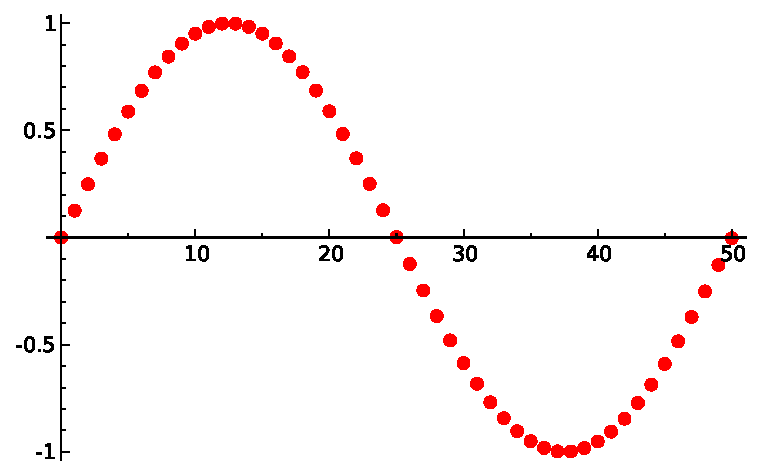
\includegraphics[width=6cm]{figures/point2d.pdf} 
\end{center}

\end{frame}

\begin{frame}{Ein Beispiel: Das Collatz Problem}

Sei $x_0\in \mathbb{N}$. Dann definiert man die folgende Folge
\[ x_n:= \left \{ \begin{array}{ll}
 x_{n-1}/2, & \mbox{falls } x_{n-1} \mbox{ gerade ist} \\
3x_{n-1}+1 & \mbox{falls } x_{n-1} \mbox{ ungerade ist} 
\end{array} \right. . \] 
Man kann zeigen, dass für alle Startwerte ein $N_0$ existiert mit $x_{N_0}=1$.
\end{frame}


\begin{frame}[fragile]{}
\begin{small}
\begin{sage}
def collatz(n):
    """ Collatz problem """
    sequence = [n]; next_value = n;
    while next_value > 1:
        if next_value % 2 == 0:
            next_value = next_value/2
        else:
            next_value = 3*next_value+1
        sequence.append(next_value)
    Objekt = point([(i,sequence[i]) for i in [0..len(sequence)-1] ]) 
    Objekt.show()   
    return sequence
\end{sage}
\end{small}
\begin{center}
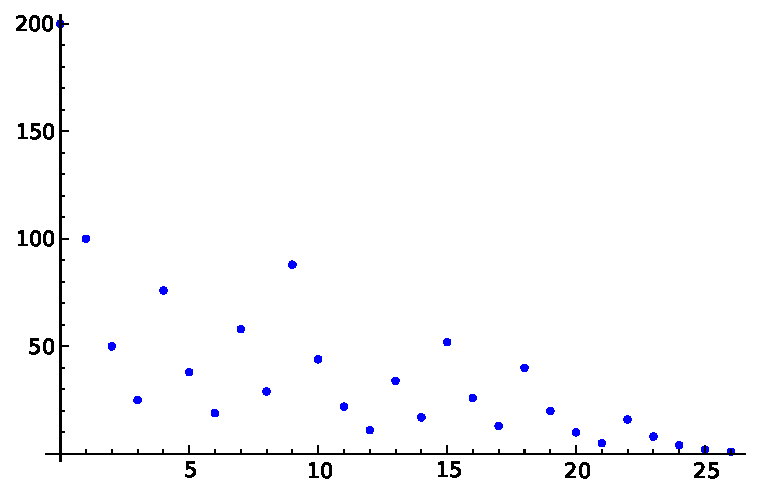
\includegraphics[width=5cm]{figures/collatz.pdf} 
\end{center}

\end{frame}

\begin{frame}[fragile]{Animationen}
mit dem Befehl \isage{animate()} lassen sich einfach Animationen erstellen. Dies funktioniert nur für zweidimensionale plots.

\textbf{Beispiel:}
\begin{sagein}
a = animate([plot(a*x^2, (x,-5,5)) for a in [-10..10]],ymin=-100,ymax=100)
a.show(iterations=1)
\end{sagein}
\begin{center}
\animategraphics[height=4cm]{2}{figures/anime_}{0}{20}
\end{center}
% \item Dreidimensionales Beispiel
% \begin{sagein}
% plotfunc3d(cos(j^0.5*PI*exp(-x^2-y^2)), 
%    x=-1..1, y=-1..1, j=1..30, Mesh=[40,40])
% \end{sagein}
\end{frame}
\end{document}
